%
% Modelo LaTeX baseado no modelo A5L
% Adaptação para LaTeX por Bruno Ferreira

% Nota: usar /newpage com 1 coluna
%       usar /clearpage com 2 colunas
%       o /newpage com duas colunas escreve na próxima coluna
\documentclass[a5paper,twocolumn, 11pt]{article}
\usepackage[landscape]{geometry}
\usepackage{indentfirst}
%Sample text
%\usepackage{lipsum}

%escrever acentos e coisas do género sem que o latex se desoriente
\usepackage[utf8]{inputenc}

%hifenização e titulos em portuguêsoa
\usepackage[portuges]{babel}

%para ter a informação de quantas páginas tem o documento
\usepackage{lastpage}

%importar cores predefinidas
\usepackage[usenames,dvipsnames]{xcolor}
\definecolor{DarkGray}{gray}{0.40}

%usar multirow e multicolumn
\usepackage{multirow}

%para ter imagens, depois define a directoria de imagens
\usepackage{graphicx}
\graphicspath{{./imagens/}}

%poder ter texto sublinhado que passa para a linha seguinte automaticamente
%usar com \uline{my underline text}
\usepackage[normalem]{ulem}

%definir o cabeçalho e rodapé
\usepackage{fancyhdr}
\pagestyle{fancy}
\fancyhead[L]{
    \small{
        \textcolor{DarkGray}{
            \textbf{Uminho 2012 - LI3 --- Transitários LEI}
        }
    }
}
\fancyhead[R]{
    \small{
        \textcolor{DarkGray}{
            \textbf{Pág. \thepage\ /\pageref{LastPage}}
        }
    }
}
\fancyfoot[C]{}

%definir regras de hifenização
\hyphenation{
chaining
Hash
}

%definir comando \hyph{}, necessário para n\hyph{}dimensionais
\def\hyph{-\penalty0\hskip0pt\relax}

\begin{document}

\onecolumn
\thispagestyle{empty}
\begin{tabular}{ll}
    \multirow{7}{*}{ 
\includegraphics[height=90pt]{logo.jpeg} }
    &\\
    & \textcolor{DarkGray}{\Large{\textbf{Escola de Engenharia}}} \\
    &\\
    & \large{Departamento de Informática}\\
    &\\
    &\\
    & \large{Licenciatura em Engenharia Informática}\\
\end{tabular}
\begin{center}
    \Large{\textbf{Projecto de Laboratórios de Informática III}}\\
    \vspace{20pt}
    \Large{\textbf{``Transistários LEI --- Projecto 2: Parte II''}}\\
    \vspace{15pt}
    \begin{tabular}{r@{, }l}
        Bruno Ferreira&A61055\\
        Daniel Carvalho&A61008\\
    \end{tabular}
    
    \vspace{5pt}
    \emph{Grupo 42}\\\vspace{15pt}
    \large{\textbf{Braga, Maio de 2012}}
\end{center}

\newpage
\twocolumn
\tableofcontents
\newpage
\listoffigures

\newpage
\section{Resumo}
Neste relatório encontram-se explicitadas de forma detalhada as decisões e implementações feitas neste projecto tendo em conta as análises de performance das estruturas de dados do \textit{Java Collections Framework} feita na etapa anterior. É também abordada a construção de uma interface gráfica em \textit{Swing} de forma a ser possível efectuar mudanças no estado da aplicação por parte do utilizador e garantir a usabilidade e acessibilidade na sua utilização.

Relativamente à aplicação em si, esta tem de garantir o manuseio de estruturas para o armazenamento de dados relativamente a utilizadores do serviço de transportes e das localidades onde existe possibilidade de efectuar serviço, a escolha da estrutura a usar recaiu sobre o HashMap. 

No seguimento deste relatório é explicado o porquê dessa escolha assim como informações da implementação do código com a interface gráfica e as opções tomadas relativamente a ambas, assim como outras decisões relevantes para o funcionamento da aplicação.


\clearpage
\section{Introdução}
O objectivo desta etapa é a construção de uma camada interactiva para a manipulação da estrutura dos utilizadores e de localidades e ligações. Torna-se então necessário desenvolver uma interface gráfica dotada de acessibilidade e opções de utilização satisfatórias de acordo com os princípios base do padrão arquitectural MVC (Model-View-Controller).
Dessa forma é pretendido que:

\begin{enumerate}
    \item{seja feita uma escolha mediante as estruturas de dados estudadas na primeira parte do projecto. A restante implementação será desenvolvida com base nessa estrutura de dados.}
    \item{se desenvolva a interface com o utilizador, em Java/Swing, que permita ter acesso às seguintes operações:}
\end{enumerate}
\begin{itemize}
    \item{carregar base de dados de utilizadores, localidades e ligações a partir de um ficheiro}
    \item{inserir o registo de um novo utilizador;}
    \item{procurar um utilizador por nome;}
    \item{procurar um utilizador por nif;}
    \item{apagar um registo por nome;}
    \item{apagar um registo por nif;}
    \item{listar todos os utilizador por palavra chave (ex: primeiro nome);}
    \item{inserir uma localidade e respectivas ligações directas;}
    \item{criar uma nova ligação entre duas localidades;}
    \item{visualizar as ligações de uma localidade;}
    \item{determinar a quantas localidades de distância está determinada localidade.}
\end{itemize}

Pretende-se também que seja feito um estudo ao desempenho de duas soluções distintas para assegurar persistência em Java: streams de texto e streams de objectos. Dessa forma, o programa deve medir os tempos para escrita e leitura (sempre dos patamares 5000, 10000, 15000 e 18000 itens) utilizando as seguintes
configurações:
\begin{enumerate}
	\item{streams de texto, para leitura (BufferedReader) e para escrita (PrintWriter)}
    \item{streams de objecto, para leitura (ObjectInputStream) e para escrita(ObjectOutputStream)}
\end{enumerate}
    


\clearpage
\newpage
\section{Conteúdo}
\subsection{Tomada de Decisões: Estruturas de Dados}
De forma a chegar a uma tomada de decisão sobre a melhor configuração em termos de estruturas de dados a usar na aplicação recorreu-se aos resultados obtidos na etapa anterior que reflectiam a performance das implementações das mesmas para a utilização e execução de operações sobre utilizadores e localidades. Abaixo seguem as configurações de estruturas de dados testadas.
Configuraçoes para localidades:
\begin{itemize}
    \item{uma estrutura baseada em ArrayList para fazer a gestão das localidades e um ArrayList para as localidades relacionadas;}
    \item{uma estrutura baseada em ArrayList para fazer a gestão das localidades e um HashSet para as localidades relacionadas;}
    \item{uma estrutura baseada em HashMap para localidades com um HashMap
para as localidades relacionadas;}
    \item{uma estrutura baseada em TreeMap para localidades com um TreeMap
para as localidades relacionadas.}
\end{itemize}

Configurações para utilizadores:
\begin{itemize}
    \item{duas estruturas baseadas em ArrayList para fazer a ordenação pelos
dois critérios: nome e nif;}
    \item{uma estrutura baseada em ArrayList para fazer a ordenação por nome
e uma estrutura auxiliar em LinkedList para a ordenação por nif;}
    \item{duas estruturas baseadas em HashMap, para guardar dados ordenados dos utilizadores;}
    \item{duas estruturas baseadas em TreeMap, para guardar dados ordenados dos utilizadores;}
\end{itemize}


\subsubsection{Utilizadores}
Na etapa anterior deste projecto, chegou-se à conclusão, através de análises à performance das estrututras de dados do Java Collections Framework, que a melhor forma de implementar a base de dados de utilizadores na aplicação seria feita recorrendo a duas estruturas HashMap, uma usando o nome do utilizador como chave e a outra usando o NIF. A vantagem do HashMap relativamente a outras configurações nota-se sobretudo em termos de inserção e procura. Tanto o ArrayList como o TreeMap tornam-se soluções menos óptimos, um pela sua falta de performance e a outra pela complexidade de inserção/remoção.

\subsubsection{Localidades}
De forma equivalente à decisão tomada sobre a estrutura para utilizadores, a escolha para a manipulação de dados relativos a localidades recai também sobre duas estruturas HashMap, sendo uma delas para localidades e a outra para as suas ligações. Isto deve-se igualmente à rapidez apresentada por esta estrutura na implementação sobre este tipo concreto de dados.
\clearpage
\newpage

\subsection{Interface gráfica}
A interface gráfica foi feita para ser concisa e simples de utilizar.

Descrevem-se agora algumas funcionalidades da interface gráfica.
\begin{itemize}
\item{Existe um menu com opções que permitem guardar e carregar o estado da aplicação ou importar dados de um ficheiro.}


\item{As várias operações sobre utilizadores ou localidades estão distribuídas por separadores. No primeiro separador, \emph{Gerir Utilizadores}, pode-se adicionar novos utilizadores, listar utilizadores existentes e remover utilizadores. No segundo separador, \emph{Adicionar Localidades}, pode-se adicionar localidades e ligações. No terceiro separador, \emph{Listar Ligações}, apenas de listam as ligações da localidade seleccionada. No quarto e último separador, \emph{Calcular Caminhos}, calcula-se o caminho mais curto entre duas localidades.}

\item{Todas as caixas de texto de pesquisa de utilizadores ou localidades funcionam num esquema de pesquisa instantânea, isto é, assim que o utilizador começa a escrever o nome de um utilizador ou localidade, os resultados começam a aparecer.}

\item{As caixas de texto de pesquisa de utilizadores ou localidades são acompanhadas de um botão que lista todos os itens.}

\item{Na tabela de utilizadores, existe um botão que permite seleccionar todos os utilizadores e um botão que apaga os utilizadores seleccionados. Antes de apagar utilizadores, é pedido ao utilizador que confirme que quer remover os utilizadores seleccionados.}

\item{No separador \emph{Adicionar Localidades}, para adicionar uma nova localidade, pode-se carregar na tecla ENTER em vez de carregar no botão \emph{Adicionar Localidade}.}
\end{itemize}

Seguem-se algumas imagens ilustrativas dos pontos acima, assim como do resto da interface gráfica.

\clearpage
\onecolumn
\newpage
\begin{figure}[h!b!t!]
    \caption[Utilizadores importados]{Utilizadores importados}
    \centering
        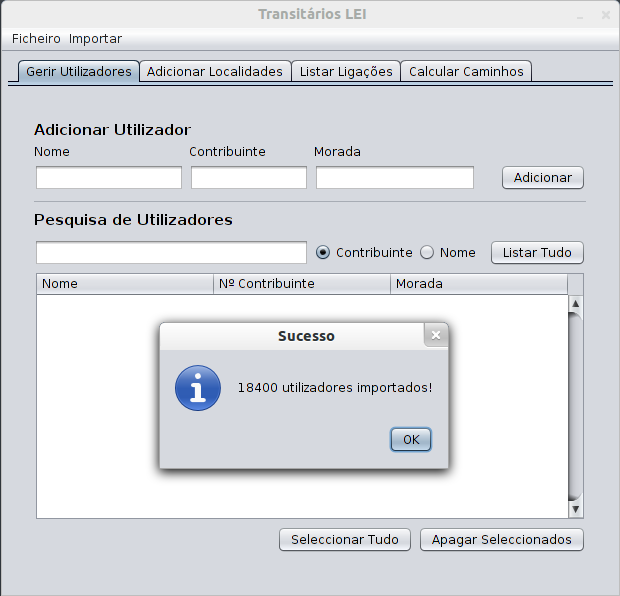
\includegraphics[width=330pt]{interface_1.png}
\end{figure}
\begin{figure}[h!b!t!]
    \caption[Utilizadores: Pesquisa]{Pesquisa de Utilizadores}
    \centering
        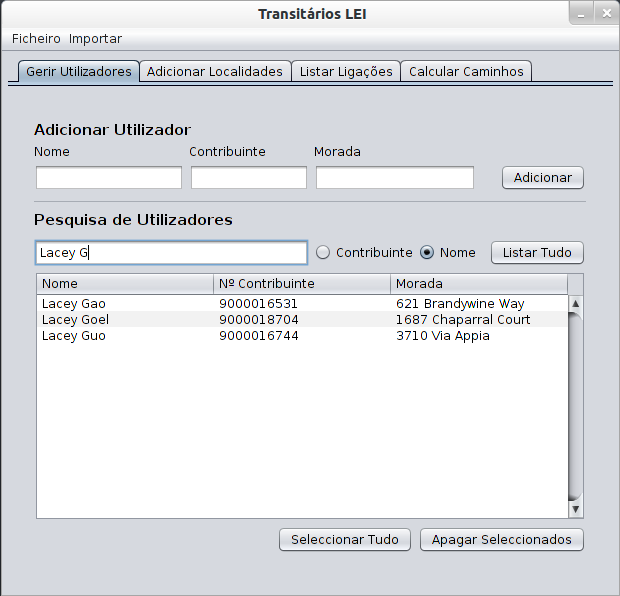
\includegraphics[width=330pt]{interface_2.png}
\end{figure}
\begin{figure}[h!b!t!]
    \caption[Utilizadores: Listar Todos]{Listar todos os Utilizadores}
    \centering
        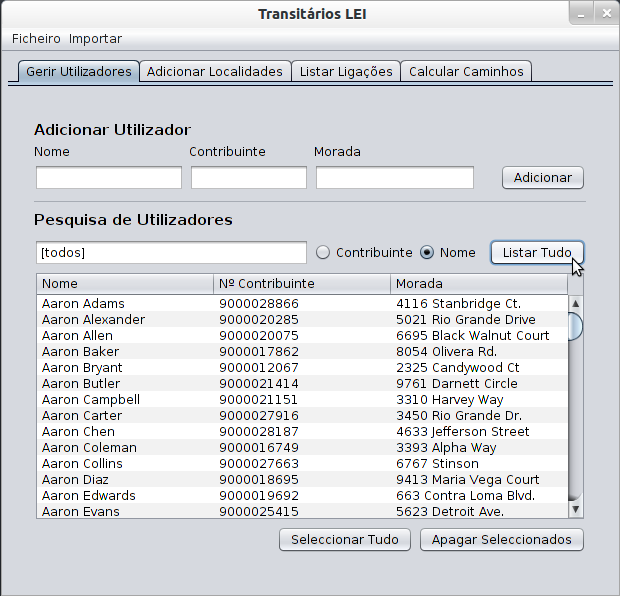
\includegraphics[width=330pt]{interface_3.png}
\end{figure}
\begin{figure}[h!b!t!]
    \caption[Utilizadores: Eliminar]{Remover Utilizadores}
    \centering
        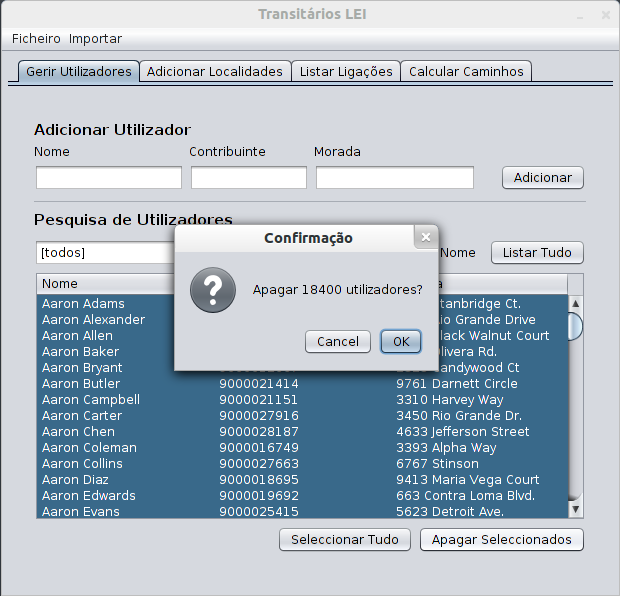
\includegraphics[width=330pt]{interface_4.png}
\end{figure}
\begin{figure}[h!b!t!]
    \caption[Nova Ligação]{Adicionar nova ligação}
    \centering
        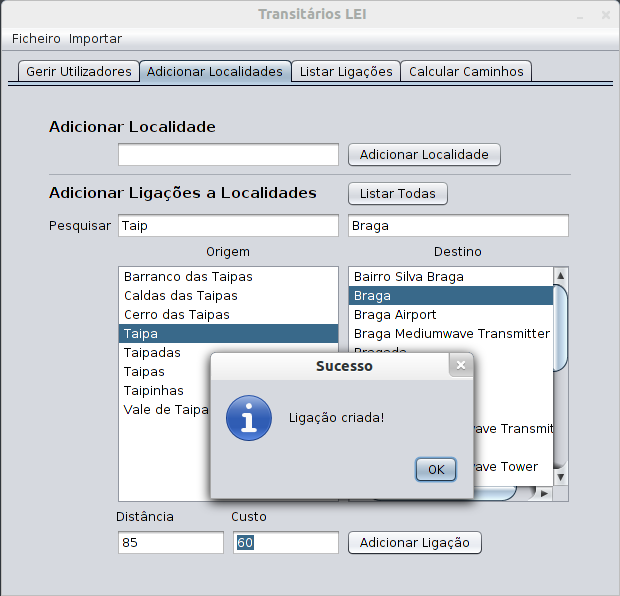
\includegraphics[width=330pt]{interface_5.png}
\end{figure}
\begin{figure}[h!b!t!]
    \caption[Listar Ligações]{Listar Ligações de Localidades}
    \centering
        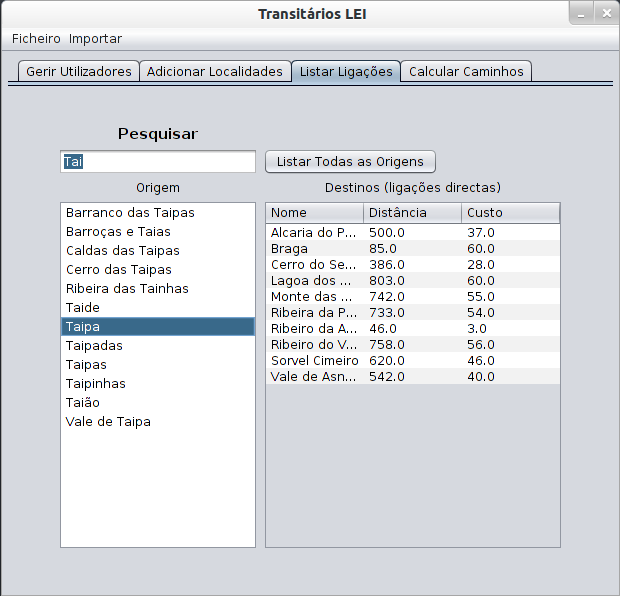
\includegraphics[width=330pt]{interface_6.png}
\end{figure}
\begin{figure}[h!b!t!]
    \caption[Calcular Caminho mais Curto]{Calcular o caminho mais curto entre duas localidades}
    \centering
        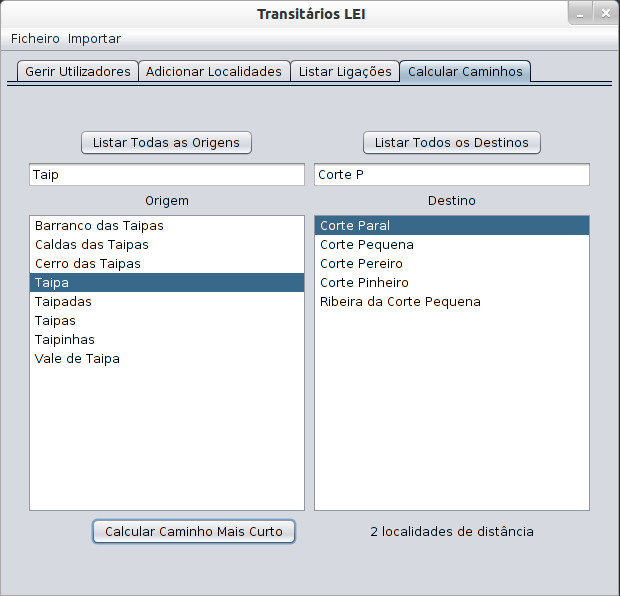
\includegraphics[width=330pt]{interface_7.png}
\end{figure}

\newpage
\twocolumn
\subsection{Camada de Persistência}
Relativamente à camada de persistência, foi pedido que se estudasse o desempenho de duas soluções distintas: streams de texto e streams de objectos.

Assegurar a persistência com steams de objectos consiste em implementar Serializable em todas as classes cujos objectos irão ser guardados. Por outro lado, para assegurar persistência usando streams de texto é necessário formatar toda a informação sobre a forma de Strings, para que essa mesma informação possa ser guardada e recuperada posteriormente consoante determinado formato.

De forma a uniformizar os resultados, todos os testes de desempenho foram efectuados na mesma máquina. As especificações técnicas dessa máquina são as seguintes:\\
\\
\begin{tabular}{ | r  | p{2.8cm} | }
    \hline
    Sistema Operativo: & Ubuntu 12.04 \\
    Modelo: & Asus G1S \\
    Processador: & \vbox{Intel Centrino} T7700 \vbox{Core2Duo} @ 2.4GHz \\
    Cache: & \vbox{2x4096Kb}\\
    RAM: & 2x1024MB DDR2 667MHz\\ \hline
\end{tabular}\\
\\

Para obter resultados consistentes, foram feitas 100 escritas e 100 leituras para cada um dos patamares pedidos em ambos os tipos de ficheiro.

Organizaram-se os resultados de escrever/ler de ambos os formatos em tabelas e gráficos. Por norma, todos os tempos se encontram em milisegundos.

De notar também que todos os gráficos obtidos aproximam a norma linear.

\clearpage
\subsubsection{Streams de Objectos}
As streams de objectos habilitam a persistência de dados com alterações mínimas no código da aplicação, mas, em contrapartida, guardam um boa quantidade de informações relativa às classes, e não aos seus dados.
Isto permite que sejam feitas uma data de verificações de consistência no momento da importação, mas também torna o processo mais demorado e o ficheiro maior. Nos testes, o ficheiro que continha 18000 utilizadores e 18000 localidades, cada uma com 8 ligações, ocupava 9.3MB.
\clearpage
\onecolumn
\begin{center}
    \begin{table}[h!b!t!]
    \begin{center}
    \caption{Tempos da utilização de streams de objectos}
    \begin{tabular}[hbt]{ | *{11}{c|} }
    \hline
        Num. & \multicolumn{2}{|c|}{escrever em ficheiro} & \multicolumn{2}{|c|}{ler de ficheiro}\\ %\hline
        Dados & $\mu$ & $\sigma$ & $\mu$ & $\sigma$\\ \hline
        5000  & 1182.88 & 122.67 & 398.6 & 43.55\\ \hline
        10000 & 3347.88 & 233.58 & 1026.92 & 92.12\\ \hline
        15000 & 6560.54 & 356.50 & 1976.44 & 234.84\\ \hline
        18000 & 9128.06 & 428.50 & 2674.32 & 357.76\\ \hline
    \end{tabular}
\end{center}
\end{table}
\end{center}
\begin{figure}[h!b!t!]
    \caption[Streams de Objectos (escrever)]{Streams de Objectos (escrever)}
    \centering
        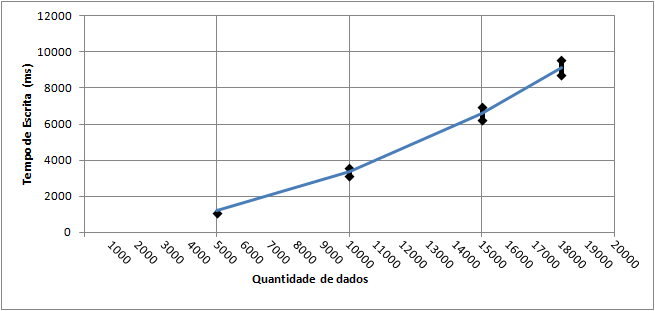
\includegraphics[width=400pt]{sdo_1.png}
\end{figure}
\begin{figure}[h!b!t!]
    \caption[Streams de Objectos (ler)]{Streams de Objectos (ler)}
    \centering
        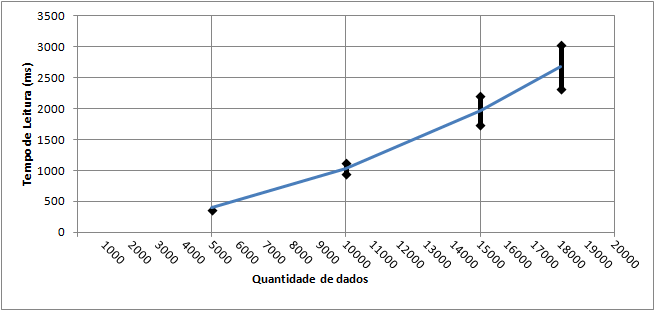
\includegraphics[width=400pt]{sdo_2.png}
\end{figure}

\newpage
\twocolumn
\subsubsection{Streams de Texto}
As streams de texto obrigam a que o código seja modificado de forma a guardar a informação formatada que permite a sua posterior recuperação.
Na recuperação dessa informação apenas podem ser feitas verificações básicas, como a verificação de tipos de dados numéricos.
Isto obriga a que, na inserção, todos os dados sejam introduzidos novamente no sistema.
Nos testes, o ficheiro que continha 18000 utilizadores e 18000 localidades, cada uma com 8 ligações, ocupava 7.5MB.
\clearpage
\onecolumn
\begin{center}
    \begin{table}[h!b!t!]
    \begin{center}
    \caption{Tempos da utilização de streams de texto}
    \begin{tabular}[hbt]{ | *{11}{c|} }
    \hline
        Num. & \multicolumn{2}{|c|}{escrever em ficheiro} & \multicolumn{2}{|c|}{ler de ficheiro}\\ %\hline
        Dados & $\mu$ & $\sigma$ & $\mu$ & $\sigma$\\ \hline
        5000 & 31.46 & 28.47 & 27.2 & 10.89\\ \hline
        10000 & 91.74 & 20.38 & 91.32 & 20.18\\ \hline
        15000 & 181.16 & 21.31 & 270.72 & 24.60\\ \hline
        18000 & 290.7 & 36.56 & 274.06 & 44.35\\ \hline
    \end{tabular}
\end{center}
\end{table}
\end{center}
\begin{figure}[h!b!t!]
    \caption[Streams de Texto (escrever)]{Streams de Texto (escrever)}
    \centering
        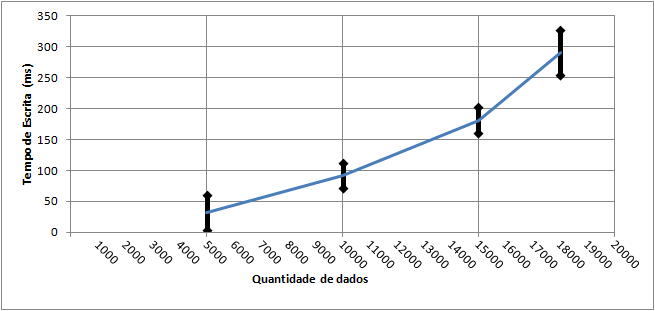
\includegraphics[width=400pt]{ef_1.png}
\end{figure}
\begin{figure}[h!b!t!]
    \caption[Streams de Texto (ler)]{Streams de Texto (ler)}
    \centering
        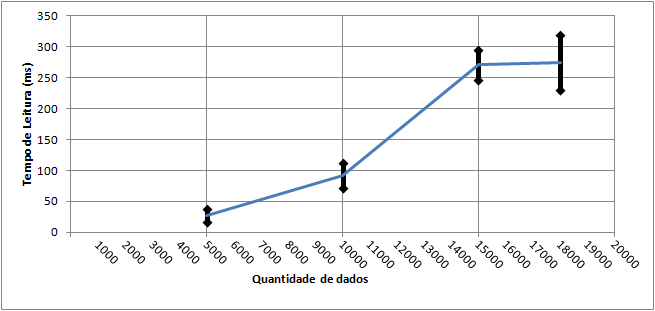
\includegraphics[width=400pt]{ef_2.png}
\end{figure}

\newpage
\twocolumn
\subsubsection{Comparação}
De ambas as configurações testadas, usar streams de texto para assegurar persistência é a mais rápida, como se pode verificar nos gráficos abaixo.
\clearpage
\onecolumn
\begin{figure}[h!b!t!]
    \caption[Comparação (escrever)]{Comparação (escrever)}
    \centering
        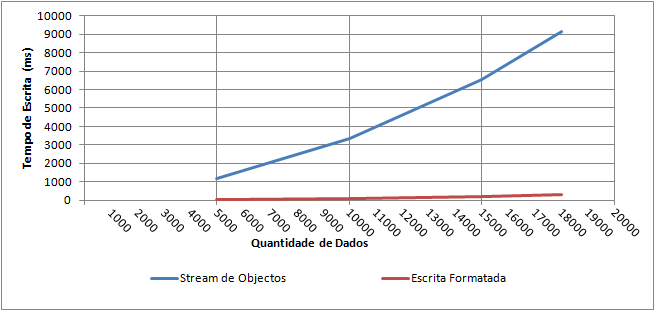
\includegraphics[width=400pt]{cmp_1.png}
\end{figure}
\begin{figure}[h!b!t!]
    \caption[Comparação (ler)]{Comparação (ler)}
    \centering
        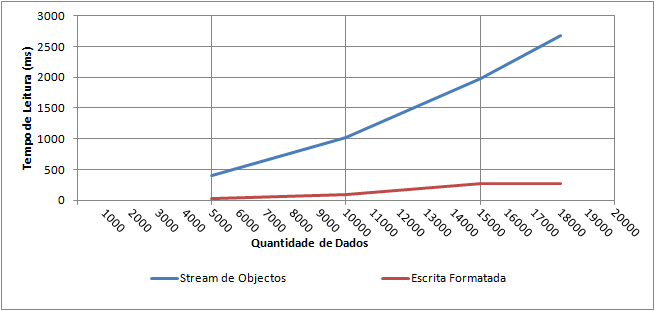
\includegraphics[width=400pt]{cmp_2.png}
\end{figure}

\newpage
\twocolumn

\clearpage
\section{Conclusão}
Com a chegada do fim deste relatório chegou a altura de se tecerem as conclusões finais. A necessidade de criação de uma interface gráfica para a aplicação foi um novo desafio, pois esta apresenta-se como a primeira oportunidade para realizar algo no que diz respeito à programação gráfica. O Swing, ferramenta primária para criação de interfaces gráficas (GUI) do Java, mostrou ser uma ferramenta de uso bastante completo, tornando necessário durante o seu uso a recorrência a pesquisas. Esta ferramenta tornou possível a criação de uma interface de uso intuitivo e completo. Tendo isso em conta pensamos ter atingido as metas deste projecto no que diz respeito ao desenvolvimento da interface gráfica.

Em termos de implementação estrutural de dados da aplicação, o Java é uma linguagem que, por ter já bibliotecas muito completas, facilita bastante a tarefa. O uso de estruturas de dados do Java Collection Framework, nomeadamente o uso de HashMap, foi bastante útil e mostrou ser a melhor forma de garantir o manuseamento da informação pedida no enunciado.

Relativamente à camada de persistência, foi-nos possível chegar à conclusão que as streams de objectos são bastante ineficientes comparativamente às streams de texto, maioritariamente pelo facto das streams de objectos guardarem dados relativos às classes que depois invocam verificações de consistência aquando da importação da informação.

Em termos gerais, consideramos que a aplicação que por nós foi construída cumpre todos os objectivos propostos para este projecto.


\clearpage
\onecolumn
\section{Fotos}
\begin{center}
    \begin{tabular}{ccc}
        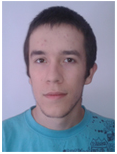
\includegraphics[width=90pt]{bruno.png}&
        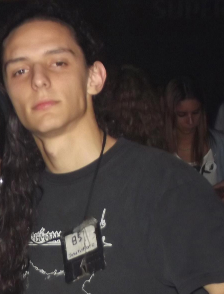
\includegraphics[width=90pt]{daniel.png}\\
        
        \small{\textbf{Bruno Ferreira}}&
        \small{\textbf{Daniel Carvalho}}\\
        \small{\textbf{A61055}}&
        \small{\textbf{A61008}}\\
    \end{tabular}
\end{center}
\end{document}